\documentclass[10pt,conference]{IEEEtran}
\usepackage[brazil]{babel}
\usepackage[utf8]{inputenc}
\usepackage{graphicx}
\usepackage{amsmath}
\usepackage{url}
\usepackage{cite}
\usepackage{float}
\usepackage{hyperref}

\title{Sistema de Monitoramento de Papel em Dispensers Utilizando Sensor Ultrassônico e Protocolo MQTT}

\author{Grupo: [Arthur Peixoto Schiller, Franc Wang e Juliana de Oliveira]\\
IBMEC - Sistemas Embarcados e IoT}\\

\begin{document}

\maketitle

\begin{abstract}
Este trabalho apresenta o desenvolvimento de um sistema protótipo para monitoramento em tempo real do nível de papel em dispensers, utilizando sensor ultrassônico e comunicação via protocolo MQTT. O principal objetivo é reduzir a insatisfação dos usuários causada pela falta de reposição, especialmente em locais com alto fluxo de pessoas. O sensor detecta o nível de papel e envia alertas automaticamente ao responsável pela manutenção sempre que valores críticos são atingidos. O sistema proposto é de baixo custo, fácil replicação e alta escalabilidade. A visualização das informações ocorre por meio de um aplicativo mobile desenvolvido com React Native.
\end{abstract}

\section{Introdução}
De acordo com o portal  ConectaExp(\href{https://conectaexp.com.br/a-era-da-experiencia-uma-jornada-de-conexao-e-transformacao/}{fonte}), vivemos atualmente na \textbf{Era da Experiência}, um momento em que as empresas, para se destacarem no mercado, precisam oferecer experiências únicas e memoráveis aos seus clientes, indo além da simples entrega de produtos ou serviços.
Nesse cenário, os consumidores tornaram-se mais exigentes, buscando \textbf{vivências significativas e marcantes} em suas interações com marcas e ambientes. \textbf{Fatores como limpeza, organização e a disponibilidade de itens essenciais} influenciam diretamente a percepção de qualidade e conforto, impactando o tempo de permanência do cliente e sua disposição para retornar.
Dessa forma, a \textbf{experiência do usuário} deixou de ser apenas um diferencial competitivo e passou a representar \textbf{um pilar fundamental para a consolidação e sucesso de qualquer negócio}.
A partir dessa observação, surgiu a proposta de desenvolver um sistema capaz de monitorar o nível de papel em dispensers utilizando um sensor de distância ultrassônico e comunicação MQTT. Ao detectar que o papel está acabando, o sistema emite um alerta, permitindo a reposição antes que o papel se esgote totalmente.

\section{Descrição do Sistema}
O sistema é composto por:
\begin{itemize}
    \item Sensor ultrassônico HC-SR04 (alcance de até 4 metros);
    \item Microcontrolador ESP32 CP2103;
    \item Comunicação via protocolo MQTT utilizando o broker Mosquitto;
    \item Aplicativo mobile desenvolvido em React Native com Expo e JavaScript;
    \item Biblioteca Paho-MQTT para integração com o MQTT;
    \item Alimentação por bateria (ainda em testes);
    \item Frequência de envio: 200 ms.
\end{itemize}

O sistema é composto por um sensor de distância posicionado no topo do dispenser de papel, responsável por medir a distância até o topo da pilha de papéis armazenados. Quando o reservatório está cheio, essa distância é mínima. À medida que os papéis são retirados, a distância aumenta proporcionalmente. Ao atingir 70\% da altura total do dispenser, o sistema interpreta esse valor como um limite crítico e emite automaticamente um alerta de necessidade de reposição.
A comunicação entre o dispositivo e o sistema remoto é realizada por meio do protocolo MQTT, segmentada em três tópicos distintos:
\begin{itemize}
    \item Porcentagem atual de papel no reservatório;
    \item Status descritivo do nível de papel, categorizado como: “cheio”, “precisa repor” ou “vazio”;
    \item Valor da distância em centímetros e sua respectiva porcentagem, transmitidos conjuntamente.
\end{itemize}
Embora a coleta de dados ocorra de forma contínua, o envio de notificações ao dispositivo móvel do responsável pela reposição é realizado somente quando uma condição crítica é detectada. Essa abordagem visa otimizar o tráfego de dados e reduzir a emissão de alertas desnecessários.

 
\begin{figure}[H]
  \centering
  \fbox{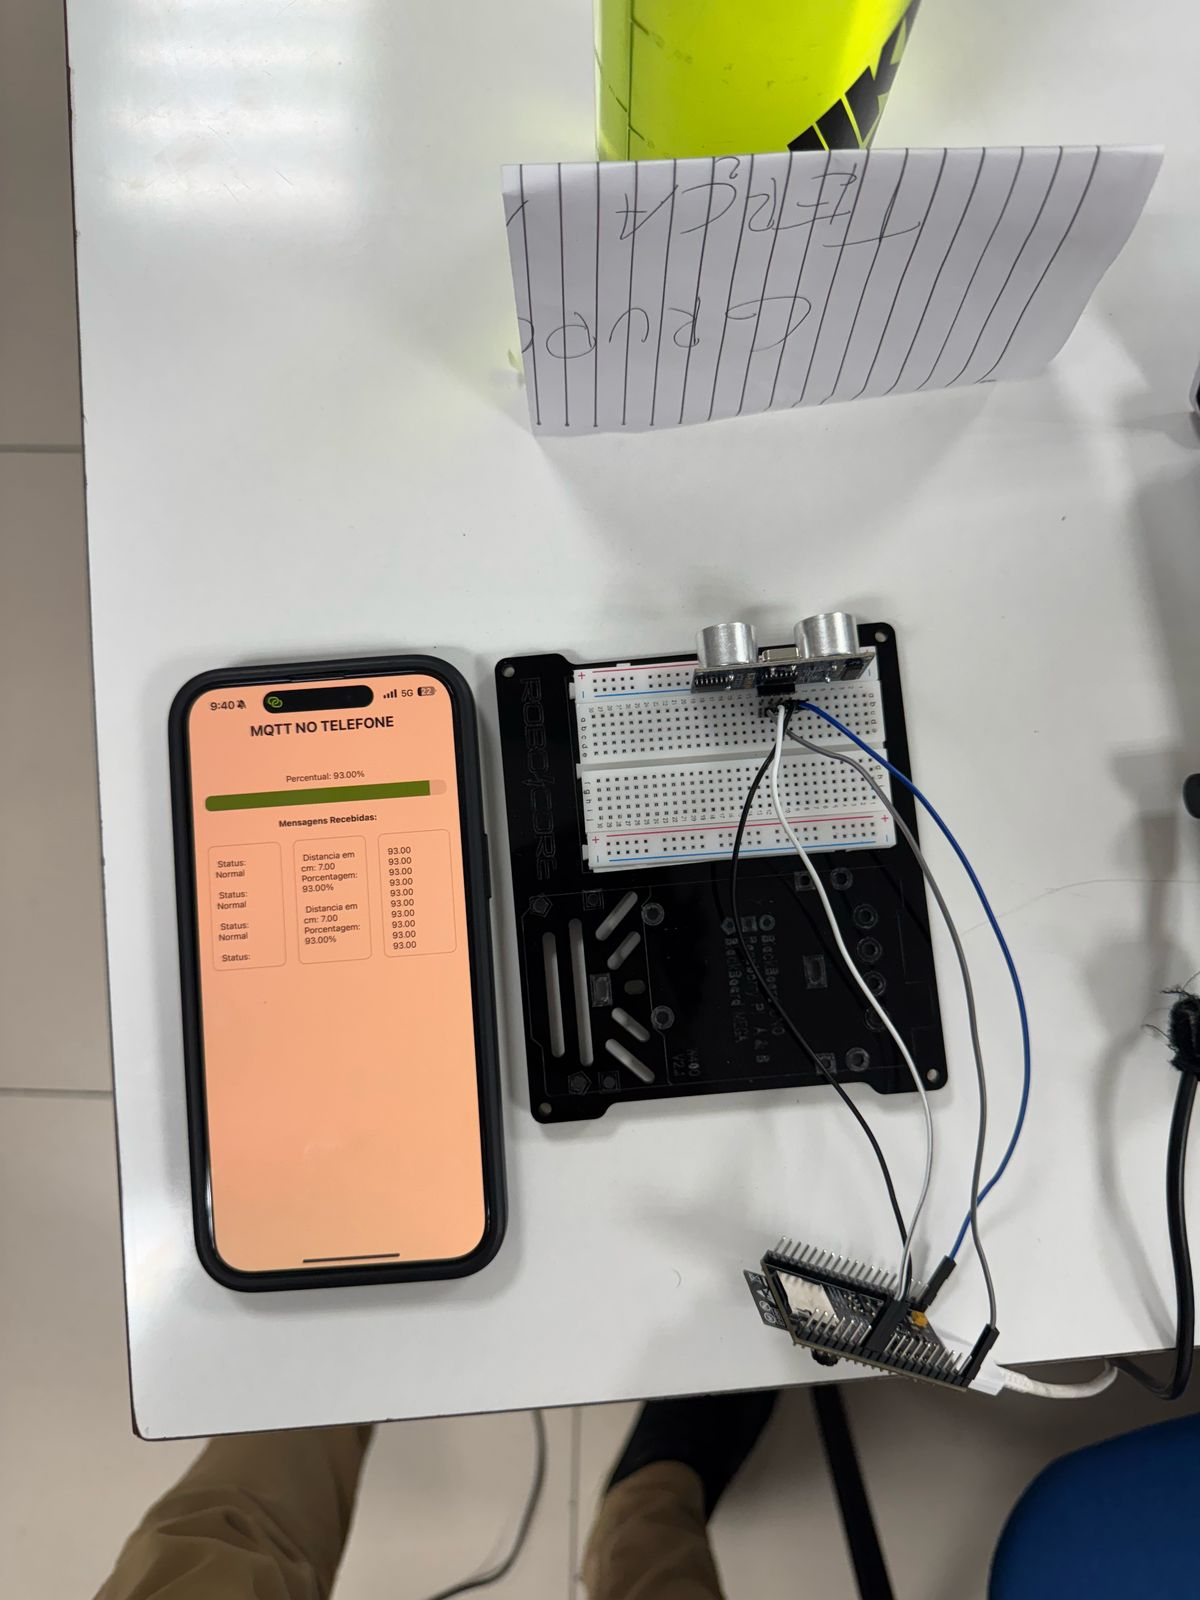
\includegraphics[width=0.4\textwidth]{montagemSistema.jpg}}
  \caption{Protótipo do sistema instalado com sensor ultrassônico e ESP montado em bancada.}
  \label{fig:sistema}
\end{figure}

\section{Análise Estatística das Medições de Distância}
\begin{figure}[H]
  \centering
  \includegraphics[width=0.5\textwidth]{medidas.png}
  \caption{Representação gráfica da análise estatística referente a quatro conjuntos de medições de distância obtidas por sensor ultrassônico.}
  \label{fig:sistema}
\end{figure}
Para avaliar a consistência e confiabilidade do sistema de medição de distância implementado, foram conduzidas análises estatísticas sobre os dados coletados durante os testes em bancada. Cada ciclo de medição possui 500 amostras e resultou em uma sequência de leituras, sobre as quais foram aplicadas as análises:

{\textbf{Distribuição das Distâncias por Medição} \\
A análise por meio de boxplots evidencia a dispersão e a presença de valores atípicos (outliers) em algumas medições. A \textbf{Medição 2}, por exemplo, apresenta maior variabilidade, enquanto \textbf{Medições 3 e 4} demonstram maior consistência e baixa dispersão. Esse tipo de visualização foi essencial para detectar leituras inconsistentes e avaliar o comportamento do sensor sob diferentes condições.

\vspace{0.3cm}
\textbf{Evolução Temporal das Leituras} \\
O gráfico de séries temporais mostra a estabilidade das leituras ao longo do tempo para cada medição. Observa-se que \textbf{Medição 3} apresenta oscilações mais significativas, enquanto \textbf{Medição 4} permanece praticamente constante, indicando uma boa resposta do sensor em condições estáveis. Essa análise temporal foi fundamental para detectar ruídos e flutuações nas amostragens.

\vspace{0.3cm}
\textbf{Média e Desvio Padrão} \\
As barras com erro (barra de erro) indicam a média das distâncias e o respectivo desvio padrão para cada medição. \textbf{Medição 2} apresenta a maior média e maior desvio padrão, indicando grande variabilidade nas leituras. Por outro lado, \textbf{Medição 3} tem média baixa com pequena variação, enquanto \textbf{Medição 4} se destaca pela estabilidade, com desvio padrão praticamente nulo. Esses dados quantificam a precisão relativa entre os testes realizados.

\vspace{0.3cm}
\textbf{Amplitude das Leituras} \\
A diferença entre o valor máximo e mínimo de cada medição revela que \textbf{Medição 2} teve a maior amplitude, reforçando a evidência de instabilidade nesse conjunto. Já \textbf{Medição 4} apresenta a menor amplitude, corroborando sua excelente consistência. A amplitude é útil como métrica de controle de qualidade e confiabilidade do sensor.

Essas análises permitiram validar preliminarmente o comportamento do sensor de distância e a integridade dos dados coletados, servindo como base para os testes em ambiente real e futuras otimizações do sistema.

\section{Testes e Validação}
Foram realizados três testes em bancada, conduzidos em ambiente laboratorial. Os resultados indicaram acurácia moderada nas medições, o que se mostrou suficiente para validar a viabilidade funcional do sistema proposto.

Como parte da arquitetura de monitoramento remoto, foi desenvolvido um aplicativo mobile com React Native que se comunica com o sistema embarcado por meio do protocolo MQTT, permitindo a visualização em tempo real do estado dos dispensadores. Essa interface web oferece uma visualização simplificada dos dados coletados, facilitando o acompanhamento contínuo e a tomada de decisão.

Direcionamento Técnico para Etapas Futuras:
\begin{itemize}
    \item Melhorias no layout da interface web, com foco em responsividade para diferentes dispositivos;
    \item Dashboard administrativo para gerenciamento de múltiplos dispositivos;
    \item Implementação de alertas visuais e sonoros para eventos críticos.

\end{itemize}
\begin{figure}[H]
  \centering
  \fbox{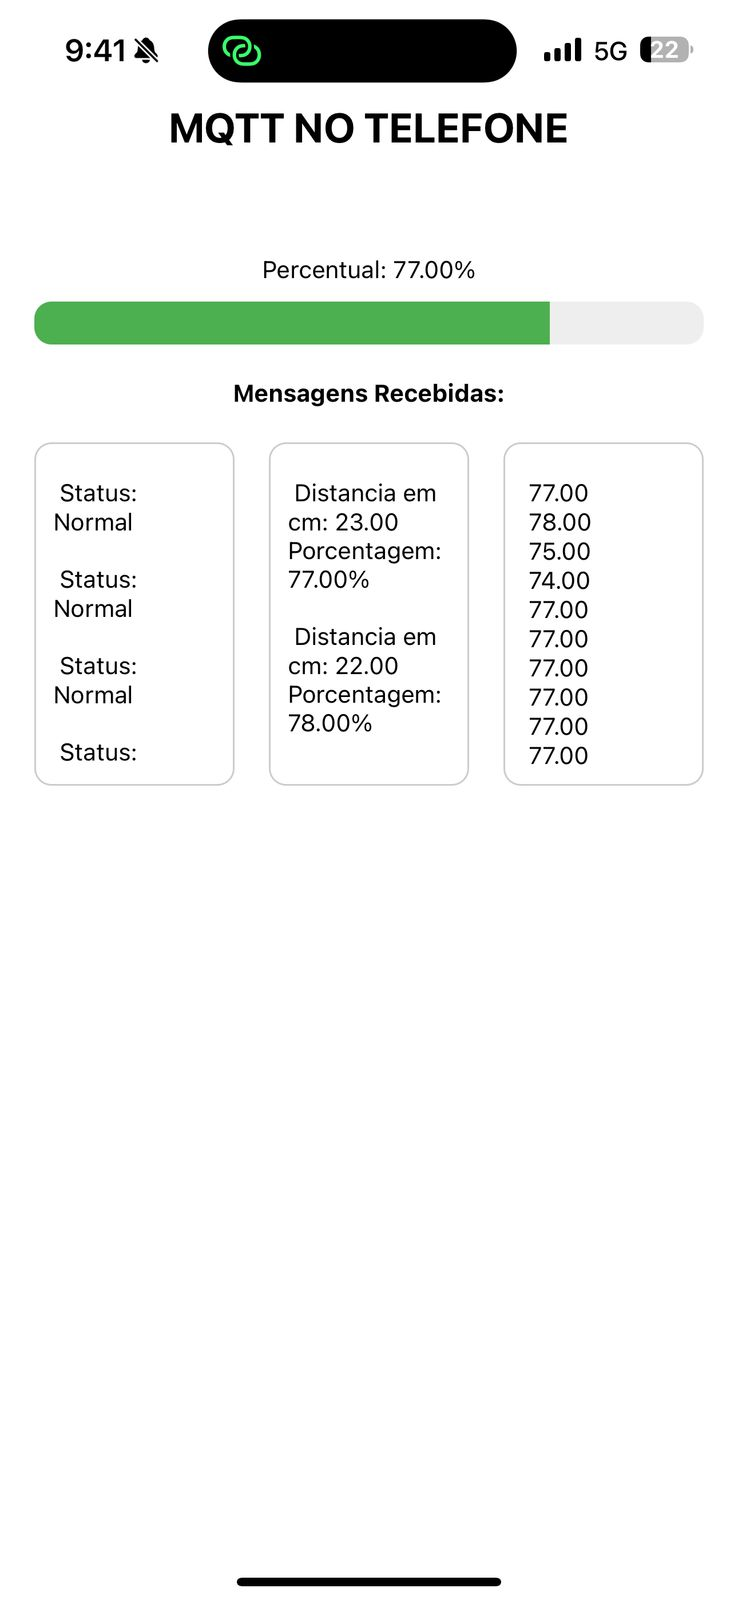
\includegraphics[width=0.3\textwidth]{printApp.jpg}}
  \caption{Tela principal do app desenvolvido para acopanhamento dos dados via MQTT}
  \label{fig:sistema}
\end{figure}





\section{Conclusão}
O sistema proposto foi submetido a testes de exatidão com o objetivo de validar sua capacidade de detectar, de forma confiável, a ausência de papel em dispensadores. Os experimentos demonstraram resultados consistentes, evidenciando a viabilidade do uso de sensores ultrassônicos para esse fim em ambientes controlados. A simplicidade estrutural e o baixo custo do projeto favorecem sua replicação e futura escalabilidade. Com a realização de testes adicionais em ambientes reais e a integração de mecanismos de segurança na comunicação de dados, o sistema apresenta-se como uma solução promissora, tanto para aplicações comerciais quanto para fins acadêmicos.Futuramente, testes em ambientes reais e aprimoramentos na segurança da comunicação de dados poderão fortalecer ainda mais sua aplicação tanto no setor comercial quanto no contexto acadêmico.

\end{document}
